\documentclass[12pt,a4paper]{article}
\usepackage[utf8]{inputenc}
\usepackage[brazil]{babel}
\usepackage{amsmath, amssymb, amsthm}
\usepackage{graphicx}
\usepackage{geometry}
\usepackage{listings}
\usepackage{xcolor}
\usepackage{hyperref}
\usepackage{float}
\usepackage{booktabs}

\geometry{margin=2.5cm}

\lstset{
  language=R,
  basicstyle=\ttfamily\footnotesize,
  keywordstyle=\color{blue},
  commentstyle=\color{gray},
  stringstyle=\color{red},
  breaklines=true,
  frame=single,
  numbers=left,
  numberstyle=\tiny\color{gray}
}

\title{\textbf{Exercício 1 -- Aula 3}\\
\large Métodos Multivariados e Machine Learning\\
PPGEST -- Universidade de Brasília}
\author{}
\date{01/2026}

\begin{document}
\maketitle

\section*{Modelo: Distribuição de Morgenstern Bivariada com Marginais Gamma}

O modelo do slide 15 é a distribuição de Farlie--Gumbel--Morgenstern (FGM) bivariada com marginais Gamma.
A CDF conjunta (slide 14, eq.\ 2) é:
\begin{equation}\label{eq:cdf}
F_{X,Y}(x,y) = F_X(x)\,F_Y(y)\big[1 + \rho\{1 - F_X(x)\}\{1 - F_Y(y)\}\big],
\end{equation}
onde $F_X \sim \text{Gamma}(\alpha,\theta)$ e $F_Y \sim \text{Gamma}(\beta,\theta)$, com $-1 \leqslant \rho \leqslant 1$.

A cópula correspondente (slide 15) é:
\begin{equation}\label{eq:copula}
C(u_1, u_2) = u_1\,u_2\big[1 + \rho(1 - u_1)(1 - u_2)\big], \quad (u_1, u_2) \in [0,1]^2.
\end{equation}

%=========================================================================
\section{Item (a): Função de Densidade}
%=========================================================================

\subsection{Derivação da PDF bivariada}

A PDF bivariada é obtida pela derivada parcial mista:
\[
f_{X,Y}(x,y) = \frac{\partial^2 F_{X,Y}}{\partial x\, \partial y}(x,y).
\]

Fazendo $u = F_X(x)$ e $v = F_Y(y)$, a CDF pode ser escrita como
\[
F = u\,v\big[1 + \rho(1-u)(1-v)\big] = u\,v + \rho\,u\,v\,(1-u)(1-v).
\]

Calculando as derivadas parciais:
\[
\frac{\partial F}{\partial u} = v\big[1 + \rho(1-2u)(1-v)\big],
\]
\[
\frac{\partial^2 F}{\partial u\,\partial v} = 1 + \rho(1-2u)(1-2v).
\]

Pela regra da cadeia, $\frac{\partial u}{\partial x} = f_X(x)$ e $\frac{\partial v}{\partial y} = f_Y(y)$, logo:

\begin{equation}\label{eq:pdf}
\boxed{f_{X,Y}(x,y) = f_X(x)\,f_Y(y)\big[1 + \rho(1 - 2F_X(x))(1 - 2F_Y(y))\big]},
\end{equation}
para $x, y > 0$, onde $f_X$ e $f_Y$ são as densidades Gamma:
\[
f_X(x) = \frac{x^{\alpha-1}\,e^{-x/\theta}}{\theta^\alpha\,\Gamma(\alpha)}, \quad
f_Y(y) = \frac{y^{\beta-1}\,e^{-y/\theta}}{\theta^\beta\,\Gamma(\beta)}.
\]

\textbf{Verificação:} Quando $\rho = 0$, a PDF reduz-se a $f_X(x)\,f_Y(y)$, confirmando a independência.

\subsection{Gráficos em R}

As Figuras~\ref{fig:contornos} e~\ref{fig:3d} mostram a PDF bivariada para diferentes combinações de parâmetros.
Os gráficos evidenciam como $\rho$ controla a direção da dependência: $\rho > 0$ gera correlação positiva (contornos alongados na diagonal principal) e $\rho < 0$ gera correlação negativa.

\begin{figure}[H]
\centering
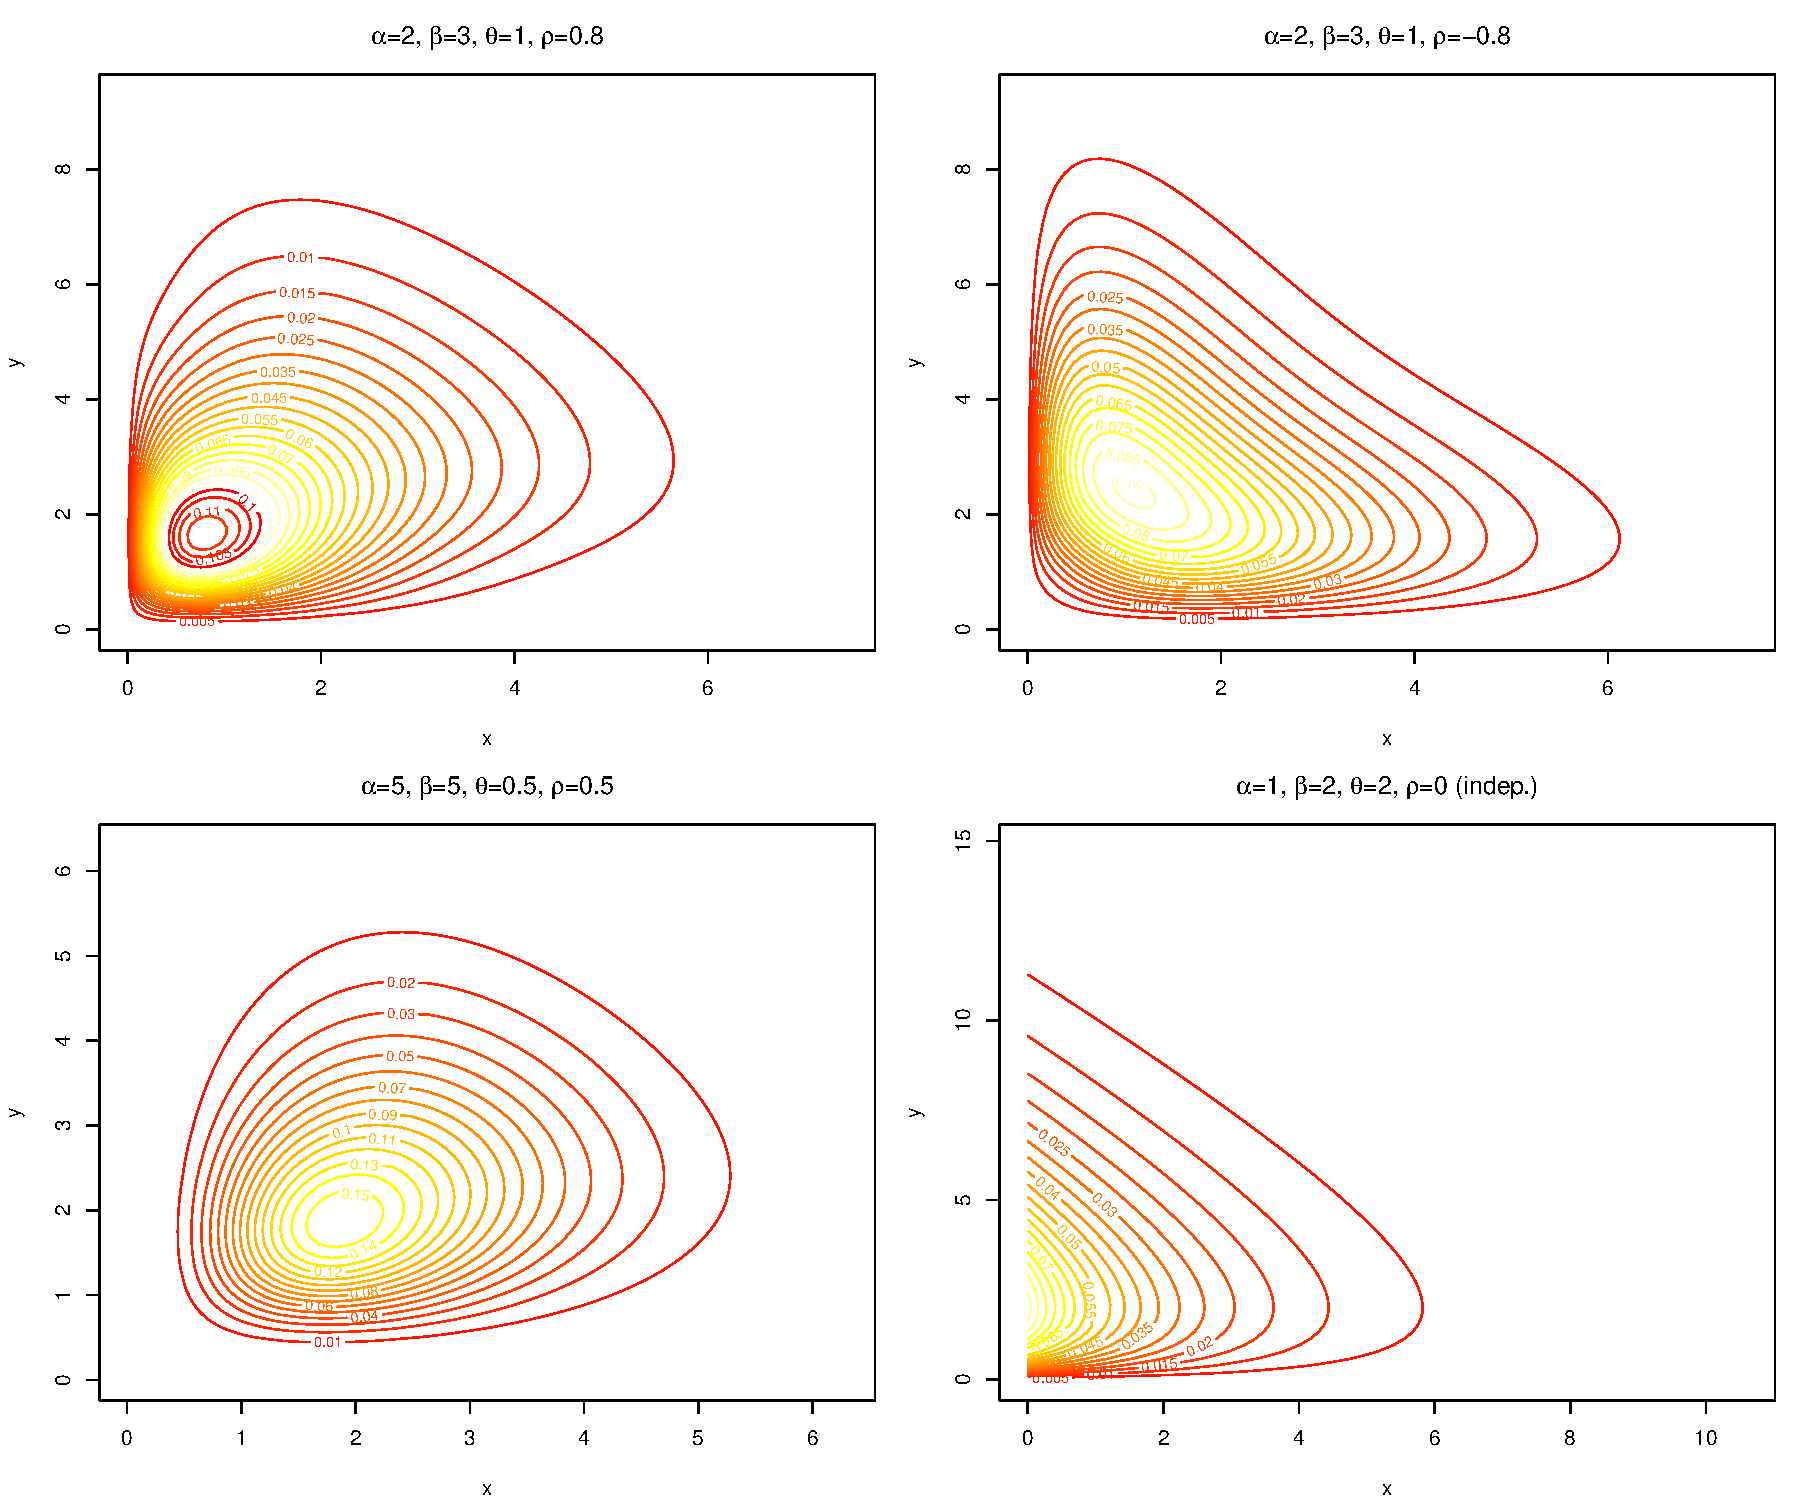
\includegraphics[width=0.95\textwidth]{plots_item_a.pdf}
\caption{Contornos da PDF bivariada de Morgenstern--Gamma para diferentes parâmetros.}
\label{fig:contornos}
\end{figure}

\begin{figure}[H]
\centering
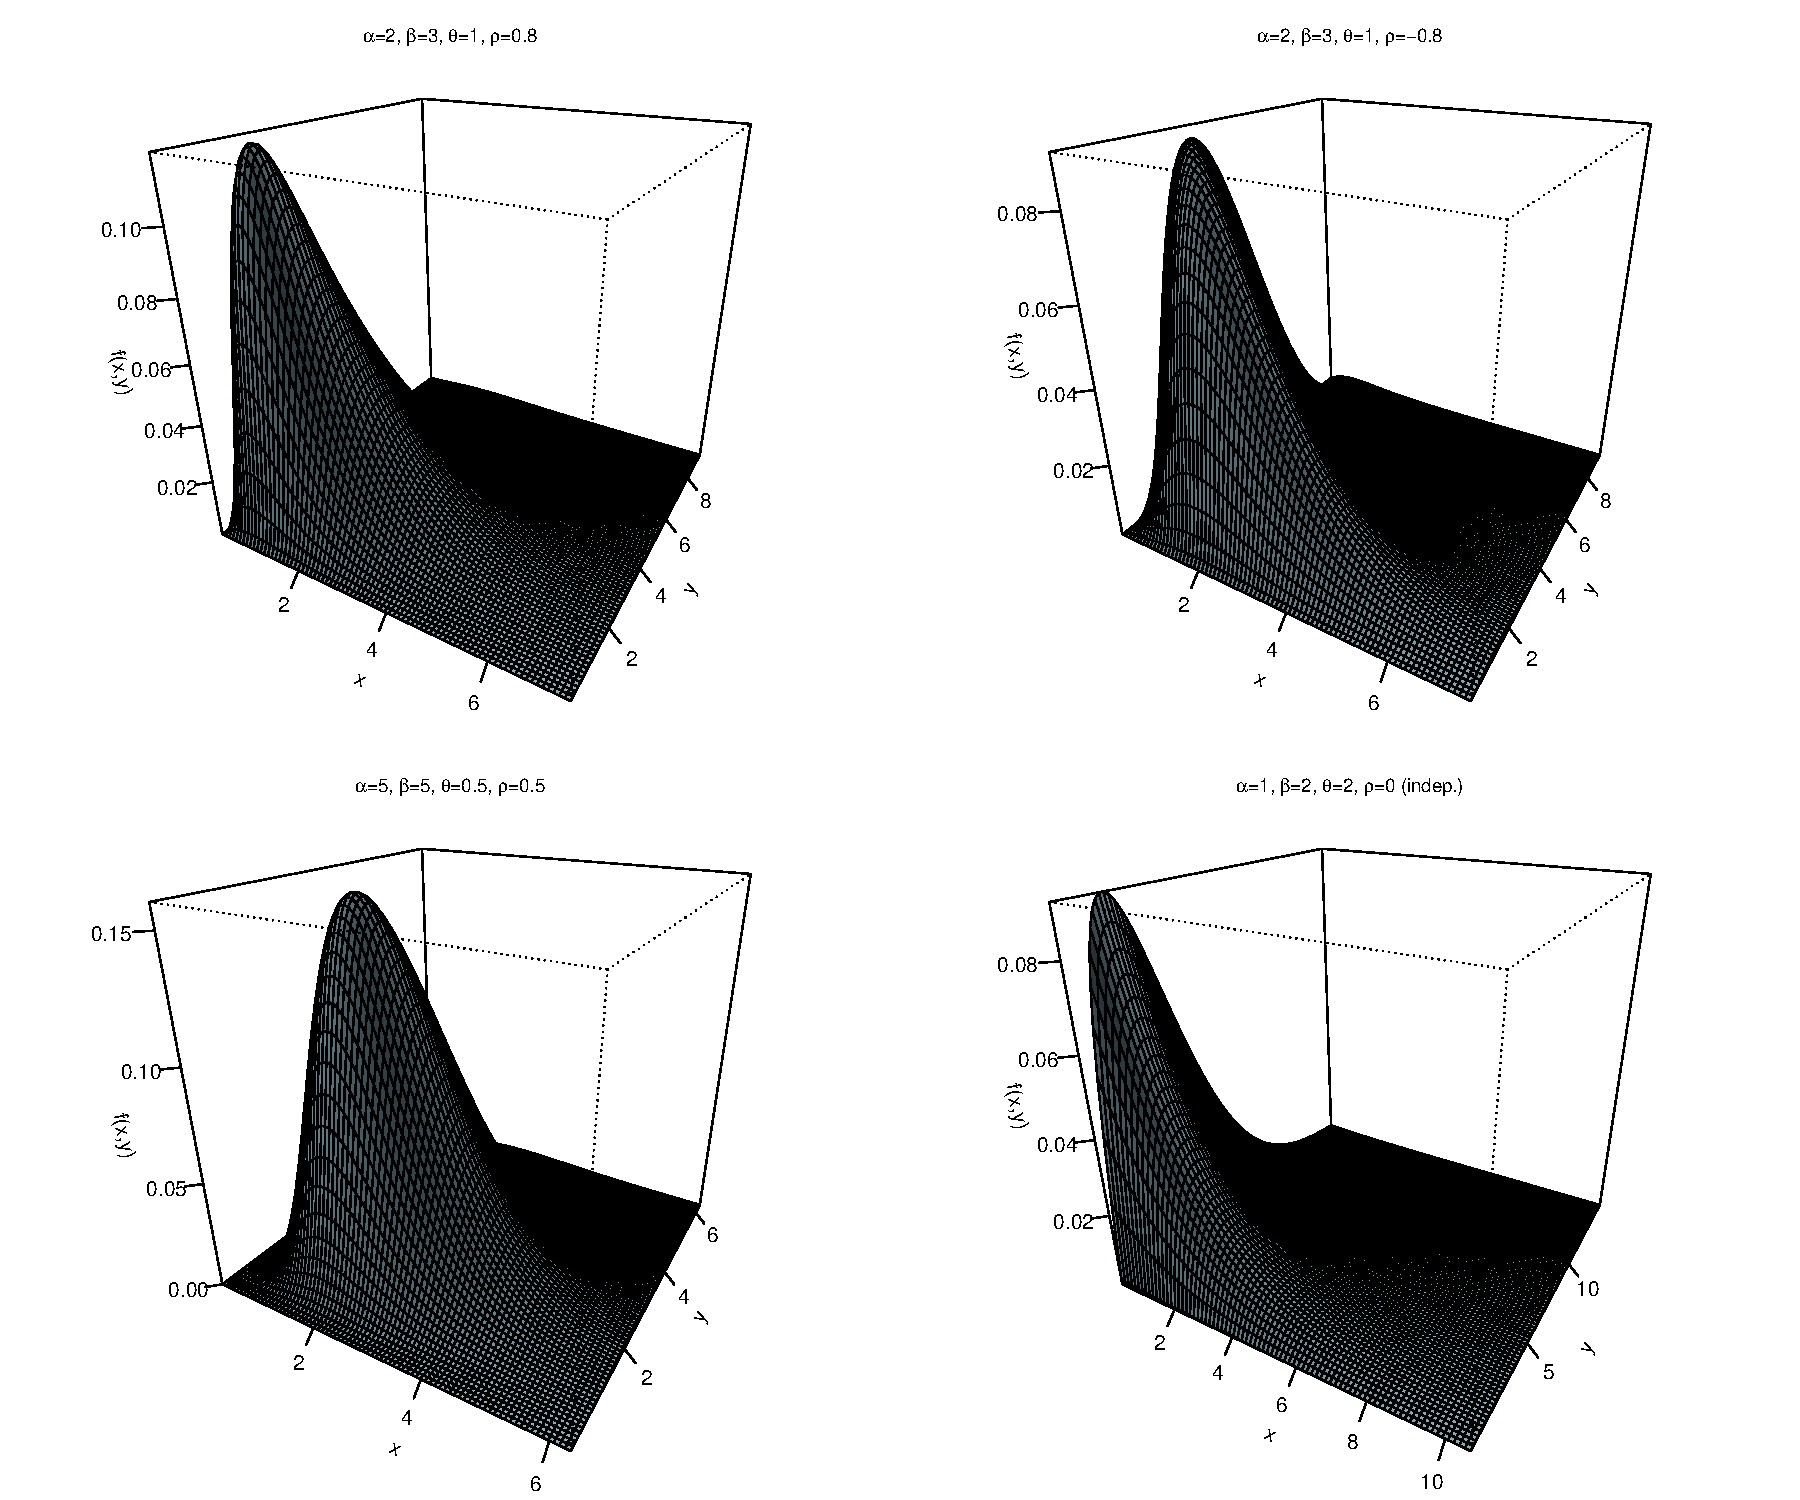
\includegraphics[width=0.95\textwidth]{plots_item_a_3d.pdf}
\caption{Gráficos 3D (perspectiva) da PDF bivariada.}
\label{fig:3d}
\end{figure}

%=========================================================================
\section{Item (b): Estimadores de Máxima Verossimilhança}
%=========================================================================

\subsection{Impossibilidade de solução explícita}

Dada uma amostra $(x_1,y_1),\ldots,(x_n,y_n)$, a log-verossimilhança é:
\begin{equation}\label{eq:loglik}
\ell(\alpha,\beta,\theta,\rho) = \sum_{i=1}^{n}\Big[\log f_X(x_i;\alpha,\theta) + \log f_Y(y_i;\beta,\theta) + \log\big(1 + \rho\,h_i\big)\Big],
\end{equation}
onde $h_i = (1 - 2F_X(x_i;\alpha,\theta))(1 - 2F_Y(y_i;\beta,\theta))$.

As equações de verossimilhança $\partial\ell/\partial\alpha = 0$, $\partial\ell/\partial\beta = 0$, $\partial\ell/\partial\theta = 0$ e $\partial\ell/\partial\rho = 0$ \textbf{não possuem solução analítica} explícita pelas seguintes razões:
\begin{enumerate}
\item A distribuição Gamma não admite EMV em forma fechada para o parâmetro de forma ($\alpha$, $\beta$), envolvendo a função digama $\psi(\cdot)$;
\item O termo $\log(1 + \rho\,h_i)$ acopla todos os parâmetros de forma não-linear, envolvendo a CDF incompleta da Gamma;
\item O parâmetro $\theta$ é compartilhado entre as duas marginais.
\end{enumerate}

\subsection{Estratégias numéricas implementadas}

Três métodos de otimização foram implementados:

\begin{enumerate}
\item \textbf{Nelder--Mead:} Método simplex, livre de derivadas. Robusto mas potencialmente lento e sem garantia de convergência ao ótimo global.

\item \textbf{L-BFGS-B:} Método quasi-Newton com restrições de caixa ($\alpha, \beta, \theta > 0$, $|\rho| < 1$). Usa aproximação numérica do gradiente, convergência mais rápida.

\item \textbf{BFGS com reparametrização:} Otimização irrestrita via transformação:
\[
\alpha = e^{\phi_1}, \quad \beta = e^{\phi_2}, \quad \theta = e^{\phi_3}, \quad \rho = \tanh(\phi_4).
\]
As restrições são automaticamente satisfeitas. Método eficiente com convergência quadrática.
\end{enumerate}

Os valores iniciais são obtidos pelo método dos momentos marginais: $\hat\theta_0 = \frac{1}{2}\big(\frac{s_X^2}{\bar X} + \frac{s_Y^2}{\bar Y}\big)$, $\hat\alpha_0 = \bar X/\hat\theta_0$, $\hat\beta_0 = \bar Y/\hat\theta_0$.

\subsection{Resultados da validação (dados simulados)}

Dados simulados com $n=500$, $\alpha=3$, $\beta=2$, $\theta=1$, $\rho=0.6$:

\begin{table}[H]
\centering
\begin{tabular}{lcccc}
\toprule
Método & $\hat\alpha$ & $\hat\beta$ & $\hat\theta$ & $\hat\rho$ \\
\midrule
Nelder--Mead & 2.9039 & 1.9294 & 1.0026 & 0.4909 \\
L-BFGS-B & 2.9039 & 1.9294 & 1.0026 & 0.4909 \\
BFGS-repar & 2.9039 & 1.9294 & 1.0026 & 0.4910 \\
\midrule
Verdadeiro & 3.0000 & 2.0000 & 1.0000 & 0.6000 \\
\bottomrule
\end{tabular}
\caption{Comparação das estimativas obtidas pelas três estratégias ($n=500$).}
\end{table}

Os três métodos convergem para o mesmo ponto. O BFGS com reparametrização foi o mais rápido (0.06s vs 0.12s).

%=========================================================================
\section{Item (c): Aplicação aos Dados de Income-Consumption}
%=========================================================================

\subsection{Descrição dos dados}

Utilizamos os dados do \textit{Survey on Household Income and Wealth} (2008) do Banco da Itália, com $Y$ (renda) do arquivo \texttt{rfam08.csv} e $C$ (consumo) do arquivo \texttt{risfam08.csv}. Após remoção de entradas inválidas, a amostra final contém \textbf{7.957 famílias}.

\begin{table}[H]
\centering
\begin{tabular}{lrrrr}
\toprule
Variável & Média & Mediana & Desvio-padrão & Correlação (Pearson) \\
\midrule
Renda (/1000) & 32,42 & 26,78 & 24,33 & \multirow{2}{*}{0,7166} \\
Consumo (/1000) & 23,84 & 20,76 & 13,78 & \\
\bottomrule
\end{tabular}
\caption{Estatísticas descritivas dos dados (escala /1000).}
\end{table}

\subsection{Resultados do ajuste}

Os parâmetros estimados pelo melhor método (BFGS com reparametrização) foram:

\begin{table}[H]
\centering
\begin{tabular}{cccc|cc}
\toprule
$\hat\alpha$ & $\hat\beta$ & $\hat\theta$ & $\hat\rho$ & AIC & BIC \\
\midrule
3,042 & 3,746 & 8,295 & 1,000 & 126.391,5 & 126.419,5 \\
\bottomrule
\end{tabular}
\caption{Parâmetros estimados e critérios de informação para os dados de income-consumption.}
\end{table}

\begin{figure}[H]
\centering
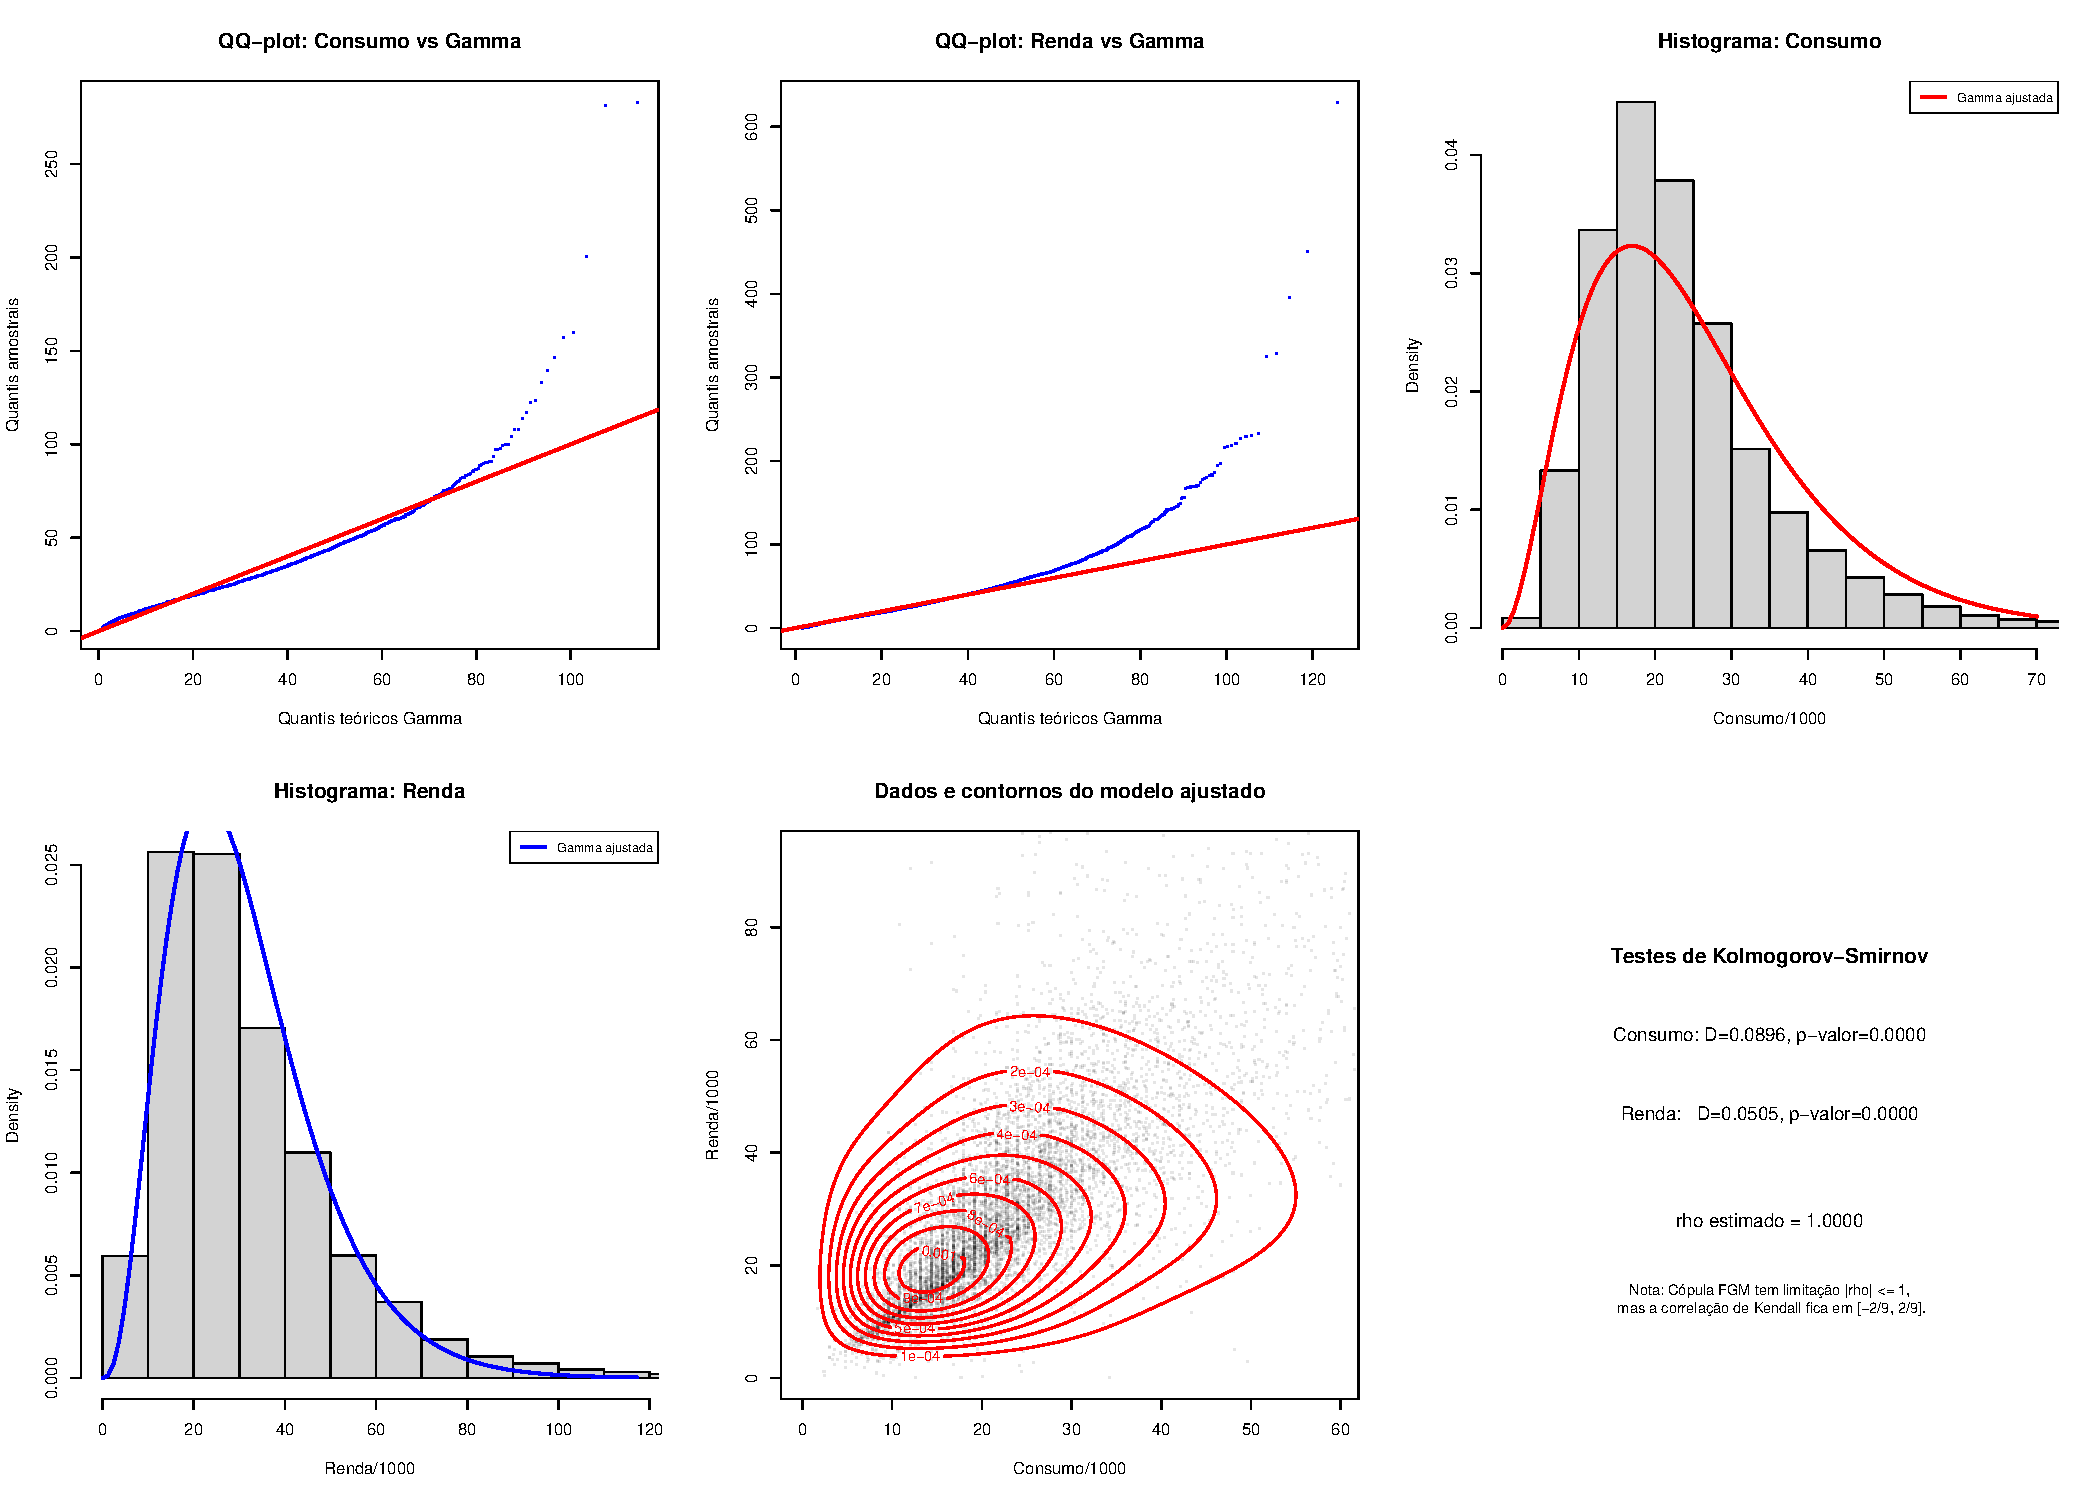
\includegraphics[width=0.95\textwidth]{plots_item_c.pdf}
\caption{Análise de qualidade do ajuste: QQ-plots marginais, histogramas com Gamma ajustada, scatterplot com contornos do modelo ajustado e resultados dos testes KS.}
\label{fig:ajuste}
\end{figure}

\subsection{Discussão sobre a adequação do modelo}

O parâmetro $\hat\rho$ convergiu para o limite superior ($\rho = 1$), indicando que o modelo \textbf{não consegue capturar adequadamente} a dependência observada nos dados. A razão fundamental é a \textbf{limitação intrínseca da cópula FGM}:

\begin{itemize}
\item O $\tau$ de Kendall teórico da cópula FGM satisfaz $|\tau| \leqslant \frac{2}{9} \approx 0{,}222$;
\item O $\tau$ de Kendall observado nos dados é $\hat\tau = 0{,}642$, que excede largamente esse limite;
\item A correlação de Pearson dos dados ($r = 0{,}717$) também indica dependência forte.
\end{itemize}

\textbf{Conclusão:} O modelo de Morgenstern bivariado com marginais Gamma é \textbf{insuficiente} para modelar adequadamente a dependência entre renda e consumo nestes dados. O $\hat\rho = 1$ na fronteira do espaço paramétrico confirma que o modelo está ``saturado'' sem conseguir reproduzir a estrutura de dependência real.

\textbf{Alternativas recomendadas:}
\begin{itemize}
\item Cópulas com maior alcance de dependência: Clayton, Frank, Gumbel;
\item O modelo Unit-Fréchet proposto por Vila e Quintino (2026), que se mostrou superior para esses mesmos dados.
\end{itemize}

\end{document}
